\documentclass[12pt,a4paper]{article}
\usepackage{times}
\usepackage{durhampaper}
\usepackage{harvard}
\usepackage{float}
\usepackage{graphicx}
\usepackage{textcomp}
\usepackage{listings}
\usepackage{amsmath}
\usepackage{subcaption}

\citationmode{abbr}
\bibliographystyle{agsm}

\title{LiDAR Surface Reconstruction for Battlefield Route Planning}
\author{Daniel Wilkinson}
\student{Daniel Wilkinson}
\supervisor{Ioannis Ivrissimtzis}
\degree{BSc Computer Science}

\date{}

\begin{document}

\maketitle

\begin{abstract}\\
  \textbf{Context/Background}\\
  When a military group is moving on foot through an area that they may not know a great deal about, they must consider the difficulty of a proposed route as well as the potential for exposure to an enemy force. Enemy movements are difficult to predict, however strategic advantage can be roughly predicted based on a finite set of factors. A LiDAR scan could be performed at relatively low cost and risk to human life to get an understanding of the terrain, and this terrain scan can be analysed to find a route that is both efficient and safe. \\
  \textbf{Aims}\\
  This project aims to utilise LiDAR data, provided by the environment agency, to find an optimal route through otherwise uncharted ground with respect to the exertion of those travelling the route, as well as the strategic vulnerabilities that the group would be subject to. This route should then be visualised in an intuitive way for non-technically literate users to understand the proposed route.\\
  \textbf{Method}\\
  To achieve these aims, I plan to create a complete reconstruction of the area through terrain reconstruction algorithms, such as cocone, and provide the user with an interface to fly through the reconstruction. To find an optimal route, I plan to develop different route planning algorithms based on Dijkstra\textquotesingle s shortest path algorithm and A* search, to find the most efficient method for this problem.\\
  \textbf{Proposed Solution}\\
  I propose a method of using A* search with several small, easily calculable heuristics in a user-defined weighting that can be changed based on situation dependent factors. This can be coupled with relatively basic computer graphics techniques to achieve an intuitive and efficient system to find the best route and brief the user on the selection.\\
\end{abstract}

\begin{keywords}
Route Planning, Surface Reconstruction.
\end{keywords}

\section{Introduction}

  \subsection{Project Overview}
  \noindent In its most basic form, this project asks ``Can a LiDAR terrain scan be used to find an optimal route through an area with regard to enemy evasion as well as traditional route optimising metrics?''. In the Afghanistan War alone, the British Armed Forces suffered 453 fatalities, \cite{op_herrick_casualties} of which 405 were killed as a result of hostile action. \cite{ops_in_afghan} In an attempt to reduce these numbers in future conflicts, this project aims to use a low-cost LiDAR scan of an otherwise unmapped area of terrain to find a suitable route between two points that will minimise the exertion on those that are trying to undertake the journey, while maintaining their personal safety by avoiding areas that would give an enemy assailant a significant strategic advantage. If this system works as intended, then the number of engagements where British Forces are at a disadvantage should decrease and when engagements do happen, the group should have more energy to efficiently fight with. To simulate war-time conditions, the LiDAR data of the UK provided by the Environment Agency will be used exclusively. \cite{env_lidar_survey} The LiDAR scans provided, like most commercial scans, consist of two separate models: a Digital Surface Model (DSM) and a Digital Terrain Model (DTM) both at 2m, 1m, 50cm, and 25cm resolution. A DSM shows the height of the highest surface, whether it be ground or another object above it, whereas a DTM shows the height of the underlying ground regardless of what is above it as is shown in Figure \ref{dtm_dsm_fig}. Coverage of England in this LiDAR scan can be seen in Figure \ref{coverage_fig}. High resolution models are only available in certain areas, however as the resolution becomes finer, more locations are null-valued, meaning even areas scanned at a high-resolution will require the use of low-resolution models to complete the terrain.

  \begin{figure}[h]
    \centering
    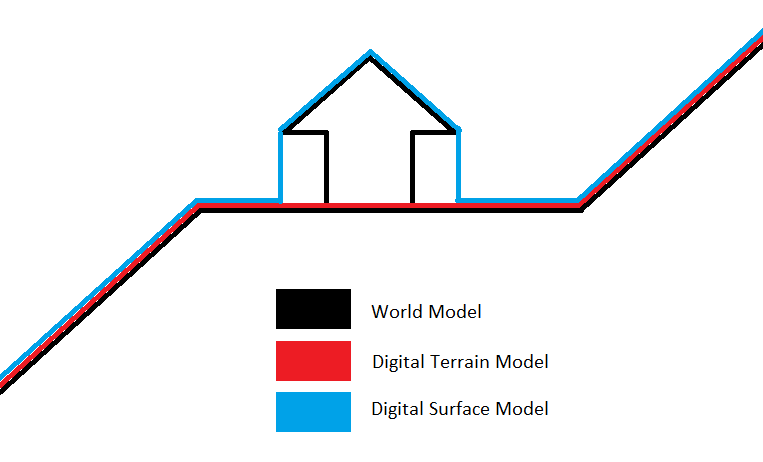
\includegraphics[width=0.75\textwidth]{dtm_dsm_diagram}
    \caption{Diagram showing the difference between DTM and DSM}
    \label{dtm_dsm_fig}
  \end{figure}

  \begin{figure}[h]
    \centering
    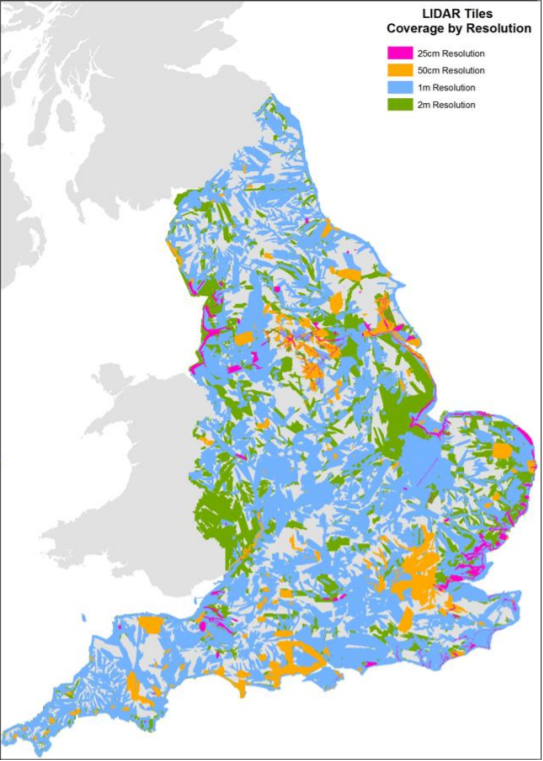
\includegraphics[width=0.55\textwidth]{lidar_coverage}
    \caption{Coverage of LiDAR scan in England, taken from \cite{env_technical_note}}
    \label{coverage_fig}
  \end{figure}

  \par Such a system will require development from many angles. Firstly, the reconstruction of the terrain from the LiDAR data will require investigation of different algorithms that claim to be able to efficiently and accurately create a mesh from point data. Once the mesh has been created, Computer Graphics techniques will need to be used to display the mesh effectively while being computationally cheap enough to run smoothly on a potentially low-powered laptop in poor conditions, such as the ruggedised laptops used by the military. A user interface will be needed that can be used by soldiers who may not be entirely literate or technologically competent, as any misunderstanding or mistakes could cost lives. In 2011, 38\% of British Army recruits had below Level 1 literacy (the minimum literacy judged to be required to function effectively in society), which is significantly higher than the UK average of 15\%. \cite{uk_literacy} Finally, and arguably most importantly, the route through the terrain must be created by the system while considering a plethora of factors outside of the standard minimum-distance route planning. The route planning element of this project must be thorough enough that it achieves the goals set out earlier, while not being overly computationally expensive, as routes may need to be found in very short timeframes to achieve a mission.

  \subsection{Stakeholders}
  \noindent This project will directly affect the lives of soldiers on the ground in current and future conflicts, as well as their commanders, who could then spend more time organising the other areas of their mission, while trusting that the system is sorting the navigation aspect for them. From a less direct perspective, this project will hopefully benefit the families of the soldiers who could have otherwise been involved in an ambush. Additionally, the taxpayers of Britain are stakeholders due to increased productivity and efficiency of our Armed Forces making taxes go further.

  \par As the developer of this system, the outcome of the project will affect me personally as it is an opportunity to increase my breadth of skill, and at the same time is my way of using my time at Durham to do something good. Once the project has come to an end, depending on my results, I may submit my findings to the Defence Science and Technology Laboratory (DSTL) to offer the system to them for further development. Therefore, while there are no current connections to DSTL, they may become stakeholders in the project at a later date.

  \par If everything goes to plan, then certain aspects of this system could be improved and adapted to be used in other applications. With a different set of parameters in the route planning section, the system could be adapted to work well in any situation from low-level flight planning to sheep herding through mountainous terrain.

  \subsection{Deliverables}
  \subsubsection{Minimum}
  \begin{enumerate}
    \item Collect data from the Environment Agency and build a document parser for their file format.
    \item Organise the collected data to be able to find all readings for same location (i.e. Surface Model, Terrain Model, multiple resolutions).
    \item Generate and render a surface mesh from the organised data.
    \item Model the surface as a graph for path generation with edge weight related to the exertion required to travel between the vertices.
    \item Generate a minimum exertion path that will take into account distance and elevation change.
  \end{enumerate}

  \subsubsection{Intermediate}
  \begin{enumerate}
    \item Recognise different types of terrain based on difference between neighbouring vertices as well as difference between surface and terrain readings.
    \item Recognise potential for cover in each area based on terrain type and features.
    \item Implement a route finding algorithm that will take cover analysis into account.
  \end{enumerate}

  \subsubsection{Advanced}
  \begin{enumerate}
    \item Model shadows on generated surface based on sun\textquotesingle s position throughout the day.
    \item Evaluate potential for silhouetting due to sun\textquotesingle s position throughout day.
    \item A selection from:
    \begin{itemize}
      \item Exit planning from high risk positions.
      \item Analysis of distance from given position to nearest safe place, or cover.
      \item Interactively input and store known enemy locations to influence probability of enemy presence in nearby areas.
    \end{itemize}
  \end{enumerate}

  \subsection{Related Work}
  \noindent Research has been done into possible parameters that can be used as heuristics when planning a route with potential enemy presence. Ruuben and Kreison suggested a set of 10 parameters which adequately allow route planning for convoys of military vehicles over well mapped areas. \citeyear{ruuben2013route} The proposed parameters for roads are: length, width, ground type, environment, road type, road infrastructure, maximum speed, maximum bearing capacity (how heavy a vehicle the road can take), units hostility (how bad the people in the area are), and threat (how likely the bad people are to attack). While some of these features, such as road type and maximum bearing capacity, do not apply to this project as we cater more towards an infantry group that are moving on a (potentially off-road) foot patrol, other features are highly transferable, such as units hostility, threat and ground type.
  \par With the possibility of using a genetic algorithm for the route planning section, Gintaras Vaira\textquotesingle s work on a genetic algorithm for the vehicle routing problem would be of great use to this project. The thesis discusses popular heuristics for the problem and proposes operators for mutation and breeding between generations and concludes that when breeding, it is more important to find common route sections from the parents and create a child from there than to take parts that appear in a single parent. Efficient pruning methods are also proposed that in testing, nearly half the number of floating point operations required. \cite{vaira2014genetic}
  \par Regarding the LiDAR surface reconstruction, work has been carried out to investigate methods of reconstructing unorganised point clouds, such as the Cocone Algorithm, \cite{DEY2011483} which works excellently, providing a reliable accurate reconstruction with boundaries. The industry standard for terrain reconstruction with organised data seems to be regular grid patterns, and work has been done to recognise buildings based on the differences between adjacent points and points on DTM and DSM. Haala, Brenner and Anders worked on urban reconstructions from LiDAR and 2D maps, with excellent results despite reducing the resolution of their LiDAR data. \citeyear{haala19983d}
  \par The routes planned in this project aim to not only protect the user from enemy interference, but also to minimise the exertion they must give to get to their destination. Minetti \textit{et al} have studied the average energy expenditure of humans while walking up or down different gradients. \citeyear{minetti2002energy} Their results can be used to approximate an expenditure function based on the difference in height between two locations. If it is possible to reliably deduce ground type based on the difference between DTM and DSM values and the difference between neighbouring values in each model, then a coefficient can be applied based on ground type to this energy expenditure to give a suitable estimate for all situations (e.g. walking uphill at  5\% gradient through forest vs walking downhill at 5\% gradient on a road).

\section{Solution}
  \subsection{Overview}
  \noindent The development of this project can be broken into 4 separate modules which can be build separately, to be used together in the final system. These are:
  \begin{enumerate}
    \item Document parser to load data from bespoke file format used by The Environment Agency.
    \item Render engine to display the LiDAR data as a surface for the user to understand.
    \item User Interface (UI) to allow the user to specify any route properties that are necessary.
    \item Route generator to model data as a graph and find the best route to take.
  \end{enumerate}

  It was decided that Java would be used as the primary development language for this project, as it provides an appropriate balance between speed of operation and simplicity to use, while also offering a high degree of cross-platform compatibility as most operating systems can run a Java Virtual Machine (JVM). As will be discussed later, extra libraries are required to enable 3D graphics rendering and UI design.

  \subsection{Document Parser}
  \noindent The data supplied by The Environment Agency uses a header to supply relevant metadata to understand the rest of the file, followed by a space separated value format where each line represents a row of the point lattice, each space denotes a column, and each value is the height of that position in metres. The header specifies the size, location, resolution, and null value of the scan, as can be seen in the example in Figure \ref{file_header}.

  \begin{figure}[htb]
    \begin{lstlisting}[language=bash]
      ncols 1000
      nrows 1000
      xllcorner    340000
      yllcorner    520000
      cellsize     1
      NODATA_value -9999
      232.7 234.55 233.16 238.89 239.29 234.1 ...
      232.22 231.93 232.54 239.06 237.43 234.08 ...
      ...
    \end{lstlisting}
    \caption{Header from a LiDAR data file}
    \label{file_header}
  \end{figure}

  \par The parser reads the file line by line, and stores the header values in private variables. Once the header has been read, a 1 dimensional vertices array is created where each set of 3 elements denotes a single point in the grid. Also created is a 1 dimensional indices array where each set of 3 elements denotes a triangle that can be easily rendered later. This method of storing the data was chosen to work easily with the render engine, as it is the most speed critical aspect of the system. Once the vertices have been loaded into the render engine, it would have been possible to create a 3D array for the data, however the calculation to find the index of the value that we want to find is simple and did not warrant the extra development and computation time to do this structure conversion.

  \subsection{Render Engine}
  \noindent To render the LiDAR data, a graphics library was required to provide a 3D world in which to display the terrain. This decision was part of the process of choosing a development language for the project. The choices were to use a high-level game engine, such as Unity, or a low-level graphics library, such as OpenGL. A game engine would make development easier as most aspects of the rendering would have already been written to a higher standard than could be written in the timescale of this project, however unnecessary extra features would also most likely be running that may slow the system down on the potentially underpowered target machines. A low-level graphics library could be more difficult to create, as all aspects would need to be made from the ground up, but the resulting system would only be running components that are entirely necessary to the project. From a personal standpoint, a low-level library would also push towards deeper understanding of graphics concepts. Consequently, it was decided that a low-level graphics library would be the better choice. OpenGL is an extremely common graphics library, however it is designed to run on Windows systems through C/C++. This project aims for a high degree of platform independence, so the LightWeight Java Game Library (LWJGL) was chosen as the library of choice. The LWJGL is a Java port for OpenGL methods, allowing similar low-level development that can be expanded on by most graphics developers if the project is continued, while running on any JVM.
  \par The Render Engine requires the vertices and indices arrays generated by the file parser, as well as points on the route generated by the rest of the system and any known enemy locations. The vertices array defines each point of the data, and the indices array specifies which points should be joined into a triangle when rendering. A visual representation of the relationship between these arrays can be found in Figure \ref{vertices_indices}.

  \begin{figure}[htb]
    \centering
    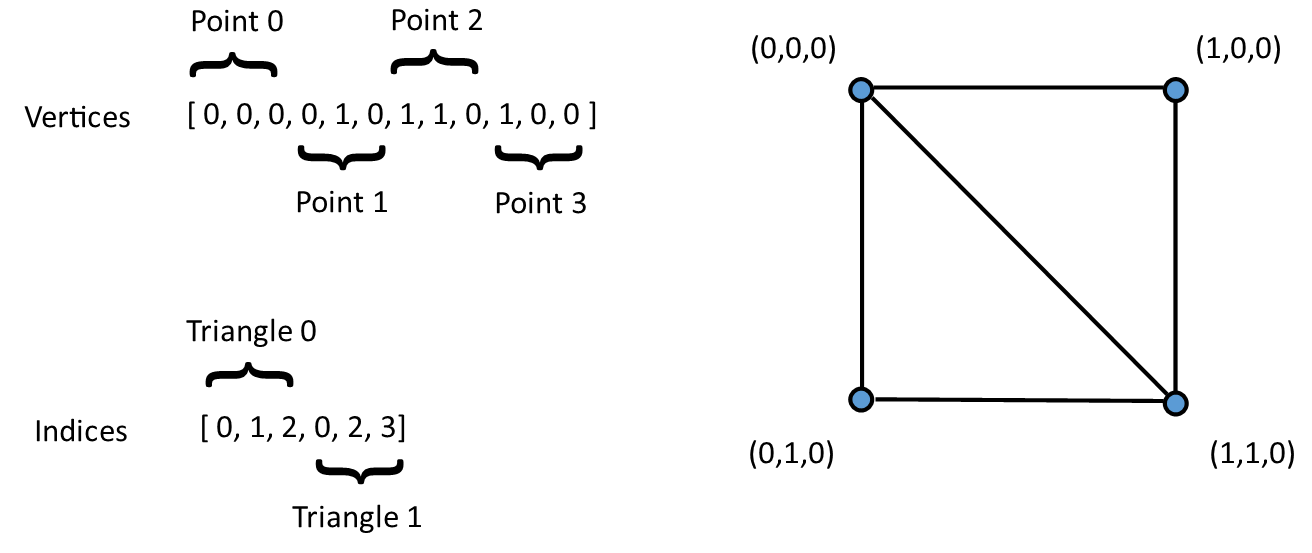
\includegraphics[width=0.75\textwidth]{vertices_indices}
    \caption{Relationship between vertices and indices array in rendering}
    \label{vertices_indices}
  \end{figure}

  The Environment Agency LiDAR scan is presented in a regular grid form, so the use of advanced reconstruction algorithms such as the Cocone Algorithm do not provide any useful improvement in output for their extra cost in computation, since it is designed to create a surface from unorganised point clouds, whereas the provided dataset uses organised points in a grid. As a result, a dot to square to triangle approach was used as is shown in Figure \ref{dot_square_triangle_fig}. Edges are created between neighbouring points to form a regular square grid across the model. Next, for each square in the grid, opposite corners are compared, and the diagonal with the lowest difference in height is selected to turn the square into two easily-rendered triangles while also providing the most natural bending point for the difficult to render 4-point polygon.
  \begin{figure}[htb]
    \centering
    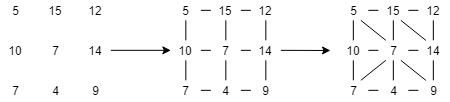
\includegraphics[width=0.75\textwidth]{dot_square_triangle}
    \caption{Visualisation for dot-square-tringle mesh generation}
    \label{dot_square_triangle_fig}
  \end{figure}

  \par Once the surface has been initially created, the colour of the vertices is decided by the use of a colour map to the vertex height. The highest point of the terrain is coloured red and the lowest point is coloured blue, transitioning through the hues as the height varies. Other methods considered for colouring were gradient colour mapping, which looked cluttered for DSM renders and sparse for DTM renders, and texture mapping, which had the potential to be misleading as it could suggest that the ground is a certain type when we do not know that it is. Texture mapping also made slight variations in height difficult to see. Height colour mapping seems to be the optimal choice for ease of understanding of terrain, although when flying through the scene close to the ground, it can be difficult to distinguish between different objects on the DSM render.
  \par After the initial colouring, the points from the route are coloured white and any known enemy locations are coloured black. This allows the user to easily tell what the proposed solution from the system is.

  \subsection{User Interface}
  \noindent Given the time scale of this project, the primary objective when selecting a User Interface creation library was to be able to rapidly develop a front end that will suffice for testing. If the project were to be put into production then much more time would need to be spent designing an interface that can be used with limited literacy skills due to the limitations discussed earlier. There is already a huge amount of research in UI design, so the focus on this project will be more towards the algorithmic side yet to be discussed. Consequently, Java Swing was chosen as the UI library as it is incredibly efficient in development time to create a working interface, and there is plenty of scope for later development into a more polished product.
  \par The design of the UI can be broken down into 4 main areas. These are the toolbar, the option panel, the route information panel and the render display. Using swing it is possible to create each panel independently and tie them all together into a single coherent display. The toolbar contains all of the buttons that control the main functions of the system. The option panel is required to specify all parameters for route selection, including the start and end point, importance of exertion and danger mitigation, resolution to use, and known enemy positions. Swing offers inputs that validate integers dependent on limits and increments specified in the code. This allows validation to be performed before any other functions are called. The render panel contains a canvas that LWJGL can access, allowing for the rendering to be in the same window as the rest of the panels. A view of the current user interface can be found in Figure \ref{user_interface}, where the toolbar is at the top, the option panel is on the left, and the rendering canvas is on the right with the route information panel beneath it.

  \begin{figure}[htb]
    \centering
    \includegraphics[width=0.9\textwidth]{../Screenshots/User_Interface}
    \caption{User Interface of system}
    \label{user_interface}
  \end{figure}

  \subsection{Route Generator}
  \noindent The main area of focus in this project was the Route Generator. Other areas of development have helped to support the usability of the system, however in an academic environment, the requirement for strong algorithmic progress outweighed the need for a pretty front end.
  \par Firstly, I needed to create a class that can take the vertices array given by the file interpreter and form a graph from the data. To do this, I chose to store the vertices array as is, since a 1 dimensional array has no excess data to store and is fast to read from, as opposed to instances of a custom position class. I then wrote methods that will calculate any desired attributes, such as the height of a position, any neighbouring points at a specified distance, and the cost of moving from one position to another, as will be discussed later. The data files used, like most LiDAR data files, have occasional null value patches where the scan has failed or the area was not scanned at all. For small patches (less than 10 metres), I chose to interpolate the values based on the values around the null patch, since a small area is unlikely to house any major dangers to the route. For any areas larger than this cut off, they remain null in the graph and are not considered in route generation. It would be irresponsible to assume that large null areas are normal ground incase there is a high risk area hidden there.
  \par The next point for development was the route itself. I chose the A* algorithm as the basis of my route finding algorithm, as it is proven that with admissible heuristics (never overestimates cost to reach goal) then A* search will return an optimal solution, and with a consistent heuristic (value for current position is no greater than step cost plus value for successor position), A* is optimally efficient.\cite{stewart_ai_search} I started to develop my algorithm by making an implementation of Dijkstra's shortest path algorithm where the weight of each edge is the flat ground distance covered plus the elevation change. When keeping track of which positions have been discovered and finalised, I chose to use ArrayLists instead of arrays set to the size of the world, as space complexity is an issue in this system, where the target computers are likely to be limited in RAM and CPU power. I decided that the potential time tradeoff was worth the extra free memory. Admittedly, this does cause a drastic change in computation time for complex routes, so I decided to implement dynamic scaling of the graph based on the `as the crow flies' distance between start and end points divided by the route resolution specified in the user interface. This cannot guarantee reasonable computation times as complex routes, where the total cost of the optimal path is high, still require a large number of points to be visited before we can be sure that we have the correct route however the mean time to compute is greatly improved.
  \par Once the Dijkstra implementation was working properly, I converted the method to use a separate cost function and use a heuristic function when deciding which node to visit next. These cost and heuristic functions could then be changed easily as the project progressed. For the heuristic function, I chose to use the `as the crow flies' distance between the current position and the end point added to the difference in height. For a minimum exertion path, this heuristic can be admissible and consistent with an appropriate cost function. For a minimum danger path, this function is not admissible, however in this system, exertion will always be an aspect of the path choice, so this is not an issue.
  \par The cost function for the algorithm is a weighted sum of two values: exertion and danger. The user is asked to assign a weight for each in the user interface, which is used in the final calculation. The exertion function is a product of the exertion to travel between the two points over open ground and a coefficient depending on the ground type. I modelled my open ground exertion function on the work of Minetti \textit{et al} \citeyear{minetti2002energy}. The graph of metabolic cost of running over gradients can be found in Figure \ref{exertion_graph}.

  \begin{figure}[htb]
    \centering
    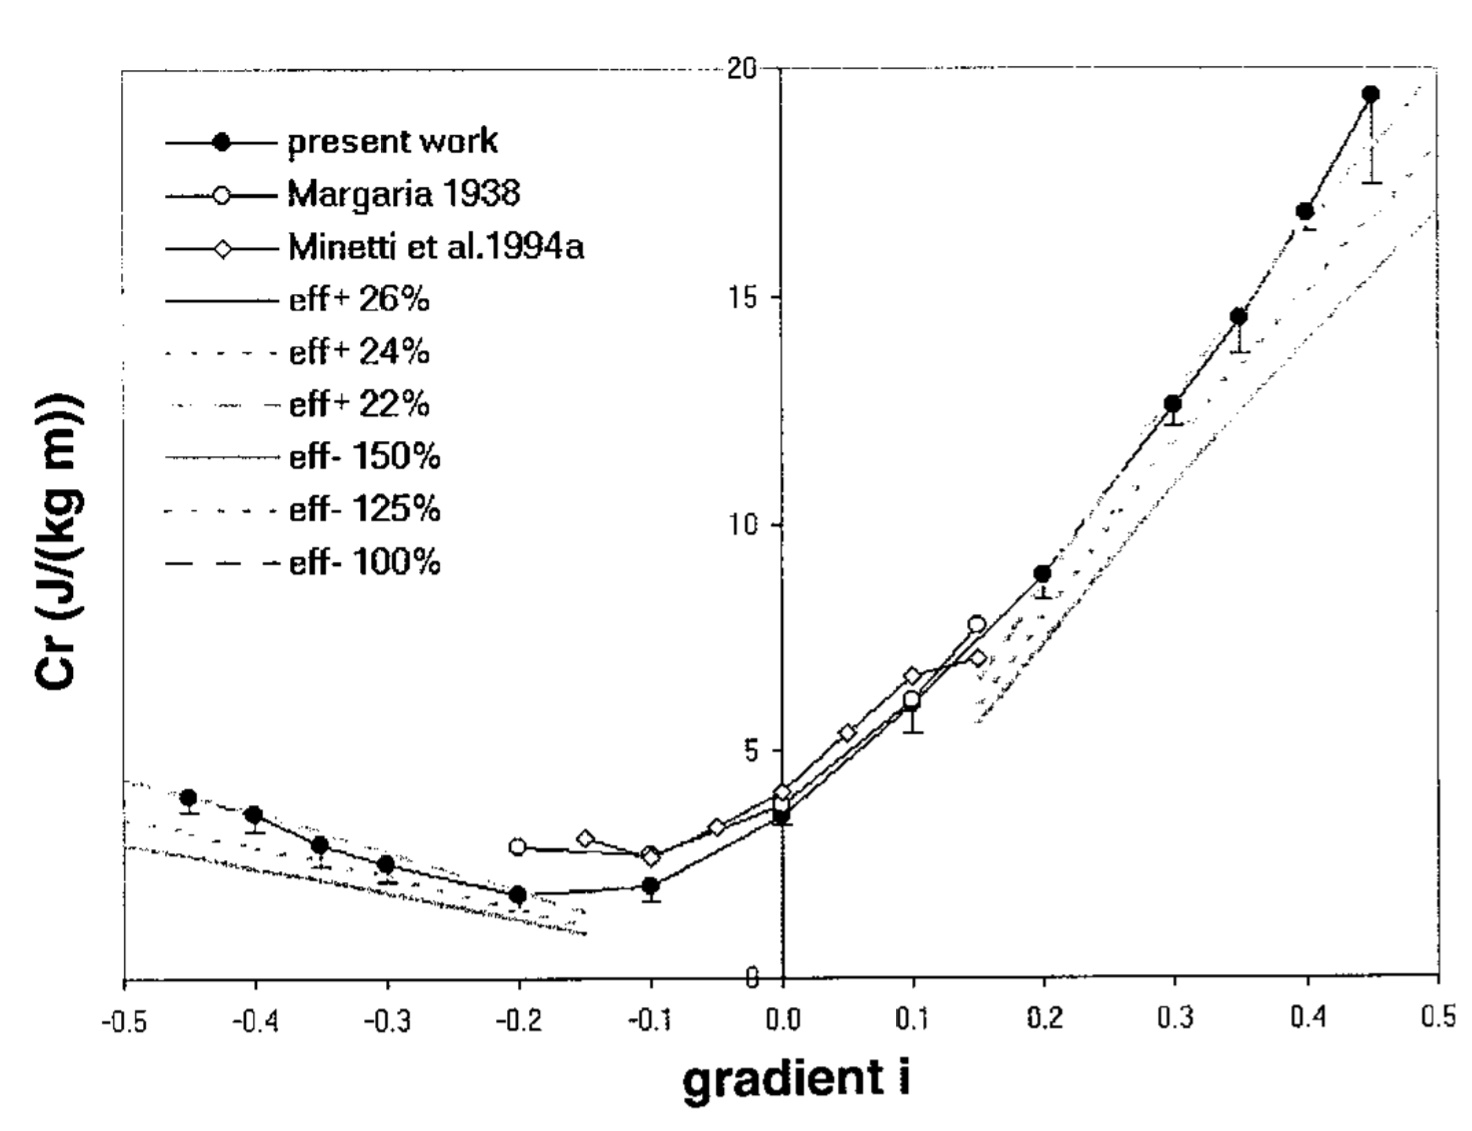
\includegraphics[width=0.75\textwidth]{exertion_graph}
    \caption{Metabolic cost of running (Cr) against gradient, as found by Minetti \textit{et al} \citeyear{minetti2002energy}}
    \label{exertion_graph}
  \end{figure}

  \par Because my system does not use Joules as the unit of exertion, the best results were found by splitting the function into positive gradients, negative gradients greater than -0.1, and negative gradients less than -0.1. I chose to calculate the exertion for a unit flat ground distance, which can then be multiplied to suit the total distance between the two points.
  \begin{equation*}
    exertion(gradient) = \begin{cases}
      100 \cdot gradient^{2} + 10 & \text{if $gradient > 0$}\\
      50 \cdot gradient + 10 & \text{if $gradient > -0.1$}\\
      -50 \cdot gradient + 5 & \text{otherwise}
    \end{cases}
  \end{equation*}

  \par I assigned the ground type coefficient by categorising the ground into open ground, forest and building as can be seen in Figure \ref{ground_types}. To determine what defines each category, I considered the difference between DTM height and DSM height. I started by finding the mean height across neighbours within 3 degrees of separation from the current position, both for surface and terrain height. If the difference in mean height is less than 1 metre, we categorise the ground as open. There is a chance that a low wall or similar object could be categorised as open ground, however due to the level of noise in real world data, reliable detection of these objects without causing false positives is a large challenge.

  \begin{figure}[htb]
    \centering
    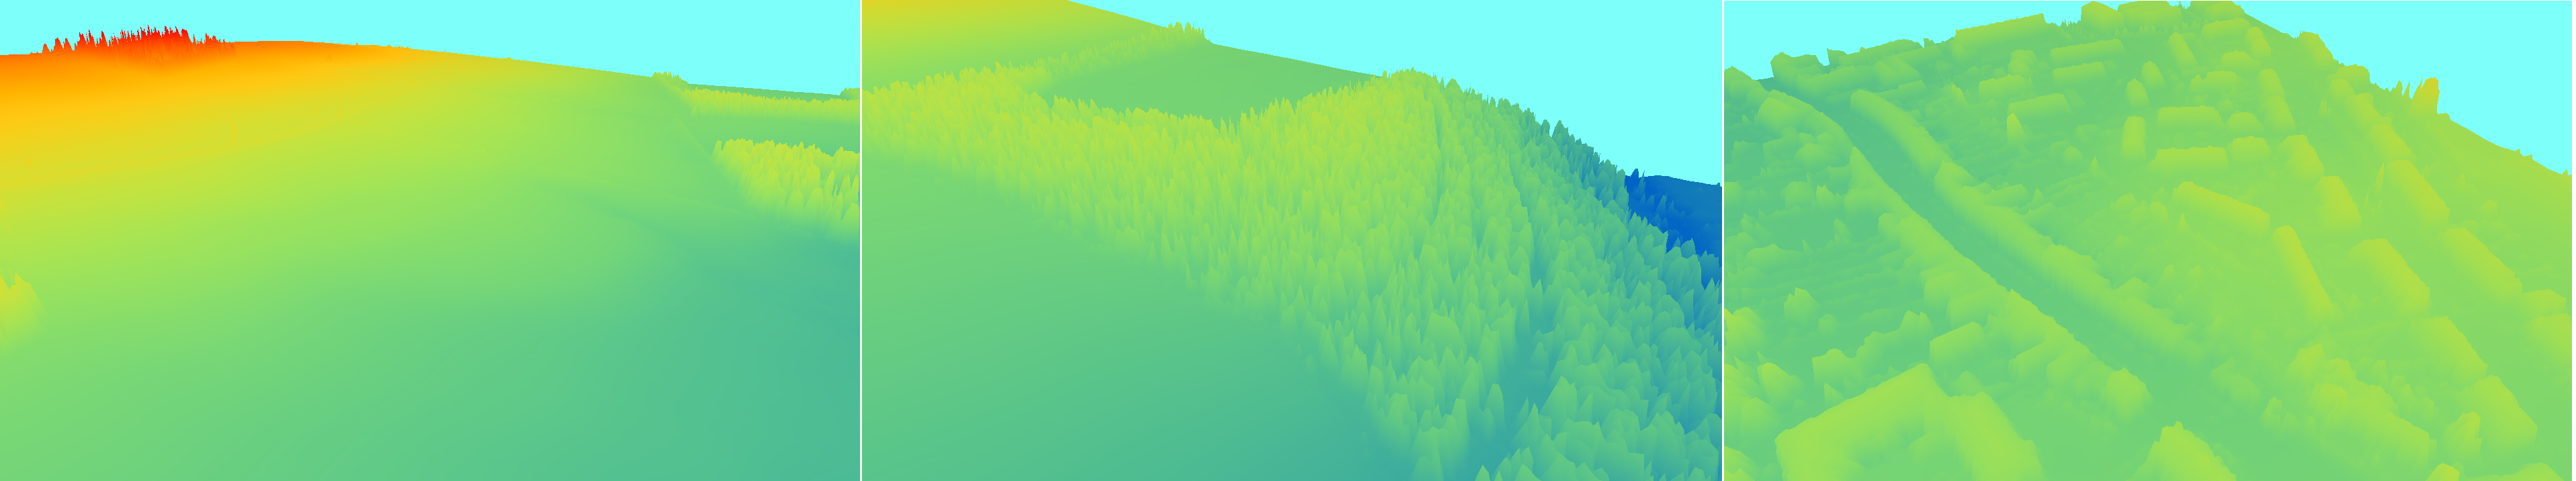
\includegraphics[width=\textwidth]{ground_types}
    \caption{Renderings of ground types. Left, open ground, and centre, forest from north west of Durham. Right, Buildings on Hallgarth St. and Whinney Hill, Durham}
    \label{ground_types}
  \end{figure}

  \par If the area is not categorised as open, then the next method of categorisation was to calculate a correlation coefficient for the DSM height inside the neighbourhood of the current position. The rationale behind this calculation is to do with the regularity of the surface; forests tend to be extremely uneven in their height, whereas buildings tend to have an even roof, regardless of orientation. To find the correlation coefficient $\rho$, I used the following equation, where $E(x)$ is the mean of $x$ in the sample.

  \begin{equation*}
    \rho = \frac{E(XYZ) - E(X)E(Y)E(Z)}{\sqrt{E(X^{2}) - E(X)^{2}}\sqrt{E(Y^{2}) - E(Y)^{2}}\sqrt{E(Z^{2})-E(Z^{2})}}
  \end{equation*}

  \par If the $\rho$ value for an area is in $-5 \leq \rho \leq 5$ then it is categorised as building, otherwise it is categorised as forest. Once the categorisation was complete, I chose coefficients for the exertion to be multiplied by to reflect the relative difficulty in moving through that terrain type. Open ground was set to $1$ as the standard for comparison. Buildings were set to $2000$ so that a route will not ask the user to gain access to a building or find a way over it unless there is absolutely no other possible way to reach the destination. The forest coefficient required testing and tweaking to strike a reasonable balance and find a good route; eventually 2.5 was found to be the optimum.
  \par Next, focus turned towards the danger cost function. Naturally, the danger cost function of a step through the graph can be broken into a sum of several other smaller calculations. The factors that are considered to contribute to the danger cost are the elevation advantage, the proximity of any known enemies, and the opportunity to get to cover if attacked.
  \par Elevation advantage stems from the difference in work against gravity that fighting sides need to do as well as the natural opportunity for cover. An extreme example would be fighting from the top and bottom of a cliff; the force at the top could peek over the top, only exposing a small area of their bodies to see the entirety of the other force, unless the people at the bottom had found suitable overhead protection. Therefore, being higher than an enemy is seen as a good thing. To find the elevation advantage, we consider the DTM height of the current position in relation to the heights of the neighbours in a larger area (7 steps in the graph). Once we know the range of heights in the neighbourhood and the relative height of the current position, we can categorise the elevation advantage of the current position using the following rules:
  \begin{itemize}
    \item If the height range is negligible (0.1 metres), then assume we're on flat ground. Here, nobody has an elevation advantage. The elevation advantage score should be neutral.
    \item If the height of the current position is among the heighest in the neighbourhood, assume we're on the summit of a hill. While we would have elevation advantage over all surrounding areas, we would be silhouetted against the skyline for assailants, and are therefore vulnerable. The elevation advantage score should be low.
    \item If the height of the current position is in the middle of the range of heights, then we're likely on a hillside. The higher up the hill, the larger the area we have elevation advantage over, with no extra likelihood of being spotted. The elevation advantage score should reflect the relative height up the hill.
    \item If the current position is one of the lowest in the neighbourhood, then assume we're in the bottom of a trough. While this can be a large disadvantage if engaged, it is easy to go undetected. The elevation advantage score should be slightly higher than neutral.
  \end{itemize}
  \par For the cost of being close to enemies, I decided the penalty should be dependent on the distance between the current position and all enemy locations. I chose the following equation, since the cost should tend to infinity if we are in the same location as an enemy, however a linear relationship would not provide a realistic balance between exertion and danger.
  \begin{equation*}
    cost = \sum\limits_{e \in Enemies} \frac{1}{distance(currentPos, e)^{2}}
  \end{equation*}
  \par The final subcalculation for danger is cover opporunity. Cover is an object or feature that can be used as a barrier to prevent being seen or block any projectiles coming from an enemy. In the LiDAR data, I have defined it as a position where the DSM is 1 metre above the DTM. To find the cover potential for a given position, I looked at the immediate neighbours, and counted the number of neighbours that satisfy the cover definition. This number is then divided by the total number of neighbours tested, and the resulting ratio is used as the position's cover score.

  \section{Results}
  \noindent The rendering of an area represents as accurately as the data allows. Comparing the rendering with a photo of the same area in the real world shows how close the representation is.

  \begin{figure}
    \begin{subfigure}{0.46\textwidth}
      \centering
      \includegraphics[width=\linewidth]{../Screenshots/real_map}
    \end{subfigure}
    \begin{subfigure}{0.5\textwidth}
      \centering
      \includegraphics[width=\linewidth]{../Screenshots/render_map}
    \end{subfigure}
    \caption{Left, Google Maps image of area near Durham.\cite{gmaps} Right, system rendering of same area.}
  \end{figure}

  \par To analyse the performance of the route finding system, we need to consider the time taken to find the route as well as the quality of the route itself. The quality of a route with regard to danger is largely subjective, so we shall discuss methods of quantifying a `good' route.

  \subsection{Time Performance}
  \noindent During testing, it became apparent that the 2 major factors that affect route generation time are the resolution chosen by the user, and the path weight of the best route to be found. A high route resolution increases the number of nodes in the graph to visit for each route, so it logically follows that the time taken to find the route will increase. A route that has a high path weight, meaning there is a large change in height, difficult ground types, or a large factor for danger, will mean that more nodes in the graph need to be expanded before we can be confident that we have the optimal route. It therefore also naturally follows that the time taken will increase.
  \par To find the effect of the route resolution on time complexity, I wrote a class to time the route finding operation of the system. I then chose a hill near Blencathra, in the Lake District to serve as my test location, asking the system to repeatedly find a route with all the same parameters, while varying the resolution value. As the resolution value affects the size of the graph in 2 directions, I would expect the time complexity to be roughly quadratic. The results can be seen in Figure \ref{resolution_time_graph}, and the predictions seem to hold well. When the resolution is kept below 100, the time to find a route is small, but quickly grows beyond 100.

  \begin{figure}[htb]
    \centering
    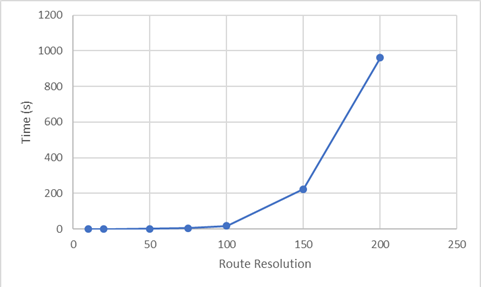
\includegraphics[width=0.75\textwidth]{resolution_time_graph}
    \caption{Graph of time to find route against route resolution.}
    \label{resolution_time_graph}
  \end{figure}

  \par The complexity of the route is more difficult to test with a single variable, however we can use intuition to say what is likely to cause a higher path weight. A complex route will primarily have large changes in altitude, with difficult ground types adding to the complexity. I tried to find areas with varying degrees of complexity and left all other attributes the same. Figure \ref{complex_time_graph} shows the effect of complexity on route finding time, as well as the associated routes with each level.

  \begin{figure}[htb]
    \centering
    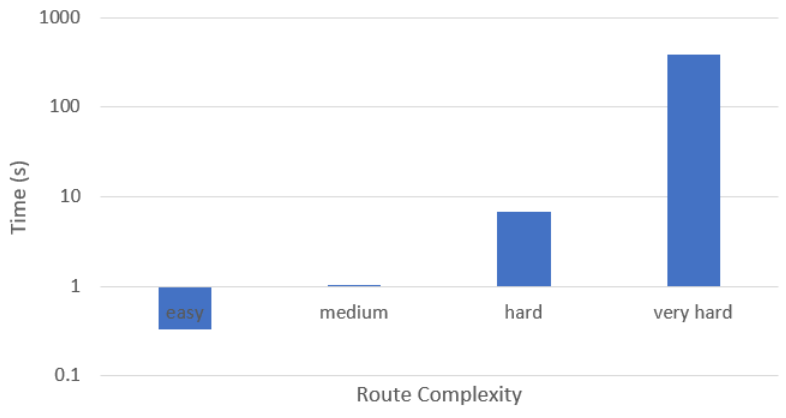
\includegraphics[width=0.75\textwidth]{route_complex_time_graph}\\
    \centering
    \includegraphics[width=0.24\textwidth]{../Screenshots/v_simple_route}
    \includegraphics[width=0.24\textwidth]{../Screenshots/simple_route}
    \includegraphics[width=0.24\textwidth]{../Screenshots/medium_route}
    \includegraphics[width=0.24\textwidth]{../Screenshots/hard_route}\\
    \centering
    \caption{Top, time taken to find route over varying complexity areas. Bottom, left to right, increasing complexity routes.}
  \end{figure}

  \subsection{Route Quality}
  \noindent The quality of a route is a highly subjective matter, so to evaluate the performance, I will compare the routes chosen by the system to the routes I would choose based on my previous training in the Air Training Corps. The analysis will be split into minimum exertion routes and routes considering danger.

  \subsubsection{Exertion only}
  To analyse the effectiveness of the minimum exertion route, we will consider the ability to avoid harsh gradients and ground types while not drastically increasing the total path length. In Figure \ref{min_exertion_avoidance:gradient}, we can see the route opting to take a longer route to get up the hill to achieve a lower, more consistent gradient to climb. A steeper section of the hill is outlined to show the disadvantage of a straight route. To test the consistency of this aspect, I made the system find 20 uphill and downhill routes with varying gradients, and attempted to find a more suitable route. The only routes that I would dispute are shallow downhill gradients, which can prioritise gradient minimisation slightly too much at the cost of total distance covered. An example route can be found in Figure \ref{failure}, where the solid white line is the route I would personally choose. All other tests were extremely positive, and any times I initially considered a separate route to be better, a valid reason to avoid it became clear upon further inspection.
  \par When asked to find a route between points that are separated by difficult ground types, the system successfully avoided buildings in all tests, and appropriately chose to avoid forests or go through them depending on how far avoiding the forest would add onto the route. I did not find any routes that I would entirely disagree with, however arguments could definitely be made against the choice to go through forests unnecessarily. If the current weightings are disliked by the eventual users, then the forest coefficient could easily be modified to suit. Examples of building avoidance and situations where forests are used and avoided can be found in Figure \ref{min_exertion_avoidance:min_exertion_avoidance}.

  \begin{figure}[htb]
    \begin{subfigure}{.5\textwidth}
      \centering
        \includegraphics[width=\linewidth]{../Screenshots/Avoiding_steep_gradient_marked}
        \caption{Gradient minimised}
        \label{min_exertion_avoidance:gradient}
    \end{subfigure}
    \begin{subfigure}{.5\textwidth}
      \centering
        \includegraphics[width=\linewidth]{../Screenshots/Avoiding_buildings_3}
        \caption{Buildings avoided}
        \label{min_exertion_avoidance:building}
    \end{subfigure}
    \begin{subfigure}{0.5\textwidth}
      \centering
      \includegraphics[width=\linewidth]{../Screenshots/Avoiding_forest}
      \caption{Forest avoided}
      \label{min_exertion_avoidance:forest_avoid}
    \end{subfigure}
    \begin{subfigure}{0.5\textwidth}
      \centering
      \includegraphics[width=\linewidth]{../Screenshots/through_forest}
      \caption{Forest used}
      \label{min_exertion_avoidance:forest_use}
    \end{subfigure}
    \caption{Minimum exertion path choices based on area}
    \label{min_exertion_avoidance:min_exertion_avoidance}
  \end{figure}

  \begin{figure}
    \centering
    \includegraphics[width=0.5\textwidth]{../Screenshots/Failed_gradient_marked}
    \caption{Arguably suboptimal route generated by system}
    \label{failure}
  \end{figure}

  \subsection{Danger and Exertion}
  The quality of the minimum danger path is also analysed by forming many paths and critically considering alternatives which could be safer. The aspects of the scenario affecting the danger value are the elevation advantage, the location of enemies, and the cover available.
  \par When the danger importance is increased, the system correctly sticks to higher ground when possible, while avoiding the summits of hills. If high ground is not possible, then very low ground is preferred, as would be expected from the coefficients specified in the solution. An example of this behaviour can be seen in Figure \ref{danger_elevation:danger_elevation}, where a low danger importance allows the system to take the shallow gradient to low ground with no unnecessary climbing. When the danger importance is increased however, the route chosen circles around the high ground of the hill before descending. It is also important to note that the route does not go too close to the hill's summit, minimising the risk of silhouetting against the skyline. Increasing the danger importance to be far greater than exertion importance does tend to cause the route to head in a straight line to the finish, however as long as values are kept reasonable, this effect is minimal.

  \begin{figure}[htb]
    \begin{subfigure}{0.5\textwidth}
      \centering
      \includegraphics[width=\linewidth]{../Screenshots/low_danger_elevation}
      \caption{Exertion weight: 1, danger weight: 1}
      \label{danger_elevation:low}
    \end{subfigure}
    \begin{subfigure}{0.5\textwidth}
      \centering
      \includegraphics[width=\linewidth]{../Screenshots/high_danger_elevation}
      \caption{Exertion weight: 1, danger weight: 2}
      \label{danger_elevation:high}
    \end{subfigure}
    \caption{Routes generated between two hills with varying exertion and danger importance weights.}
    \label{danger_elevation:danger_elevation}
  \end{figure}

  \par If we add a single or multiple enemies, the system put as much distance between the route and the enemy as possible without significantly increasing the total length of the route. In Figure \ref{danger_enemy:danger_enemy}, we can see the effect of enemies (shown as black dots on surface) on a route through a set of buildings as the number of enemies increases. The key point to note is that if there is no way to easily reach the finish without passing nearby an enemy, the route will loop around and find a much longer but safer way.

  \begin{figure}
    \begin{subfigure}{.5\textwidth}
      \centering
      \includegraphics[width=\linewidth]{../Screenshots/Avoiding_buildings_3}
      \caption{0 enemies}
      \label{danger_enemy:zero}
    \end{subfigure}
    \begin{subfigure}{.5\textwidth}
      \centering
      \includegraphics[width=\linewidth]{../Screenshots/Enemy_in_buildings}
      \caption{1 enemy}
      \label{danger_enemy:one}
    \end{subfigure}
    \begin{subfigure}{.5\textwidth}
      \centering
      \includegraphics[width=\linewidth]{../Screenshots/multi_enemies}
      \caption{2 enemies}
      \label{danger_enemy:two}
    \end{subfigure}
    \begin{subfigure}{.5\textwidth}
      \centering
      \includegraphics[width=\linewidth]{../Screenshots/3_enemies}
      \caption{3 enemies}
      \label{danger_enemy:three}
    \end{subfigure}
    \caption{Route through same area with varying number of enemies.}
    \label{danger_enemy:danger_enemy}
  \end{figure}

  \par The cover analysis seemed to have a better effect than I expected. By seeking to minimise the value for cover analysis, the system appears to avoid open spaces as much as possible, opting instead to extend the length of the route and skirt around the side of forests or built up areas. This is a highly desirable trait for the route to possess as it is easy to spot movement across an open area, leaving the group vulnerable. Moving next to a forest or other cover masks the movements of the group as well as offering protection in a firefight, while not causing the extra exertion of travelling through the forest. In Figure \ref{danger_cover:danger_cover}, we can see an example of such behaviour. The route does not go directly to the forest, however it choses a route that is a compromise between exertion and danger, as would be expected.

  \begin{figure}
    \begin{subfigure}{0.5\textwidth}
      \includegraphics[width=\linewidth]{../Screenshots/cover_no_danger}
      \caption{Danger not considered}
      \label{danger_cover:no_danger}
    \end{subfigure}
    \begin{subfigure}{0.5\textwidth}
      \includegraphics[width=\linewidth]{../Screenshots/cover_danger}
      \caption{Danger considered}
      \label{danger_cover:danger}
    \end{subfigure}
    \caption{Routes through same area with and without minimisation of danger.}
    \label{danger_cover:danger_cover}
  \end{figure}

  \section{Evaluation}
  \par In general, the system works well to find a route based on the amount of computational power available. Upon further testing and research, extra metrics for route quality could easily be added to the cost and heuristic functions, improving the route based on a user's personal route preferences. The vast majority of routes generated match my preferred route almost exactly, however as a large stakeholder, there is the possiblity that I have an unintentional bias in my analysis.

  \par The A* based algorithm used in this project seems to work well for the application. Minimal routes for exertion are found in most cases, with very few exceptions, as was explored in the results. Minimal danger routes are found as long as user defined parameters are kept proportional, based on my interpretation of what comprises a safe route. It is important to note that since the system was built around my route preferences, there may be a bias in how I percieve the quality of the results. To account for this bias, the A* cost function can be easily adapted to suit the needs of future users if they have different priorities in route selection. The calculations used to determine the danger cost were, in my opinion, a good compromise between required computational power and accuracy. Attempts were made to create a simulation of the sun's light and resulting shadows, coupled with ray picking algorithms to detect exactly where the current position was visible from. This was not achievable in single thread processing while maintaining a reasonable level of performance. With much more time, it may be possible to develop a system using OpenGL to simulate the scenario and retrieve any necessary data from a rendering that is not displayed to the use. To store the necessary data for each position at each point in the day would be enormously expensive in space, however to generate the data while considering a route would be equally computationally expensive, even when the computation time is minimised by using a GPU.
  \par To make the system ready for use on frontlines, the route alterations mentioned above are not strictly necessary; the route generation currently implemented is more than adequate for initial trials. The main development required with more time would be working on the user interface to allow soldiers with limited literacy to input route parameters more easily. The actual route should be easily interpreted as the system stands, as a realistic rendering of the area is shown with the route clearly shown in white and enemies in black.


%
% \section{Design}
%
%   \subsection{Requirements}
%   \noindent After analysing the deliverables set out above and considering the possible use cases of the system, as can be seen in the use case diagram in Figure \ref{use_case_diagram_fig}, this section will define the system\textquotesingle s functional requirements in Table \ref{fr_table} and non-functional requirements in Table \ref{nfr_table} as well as ranking each requirement on its importance to the final product.
%
%   \begin{figure}
%     \centering
%     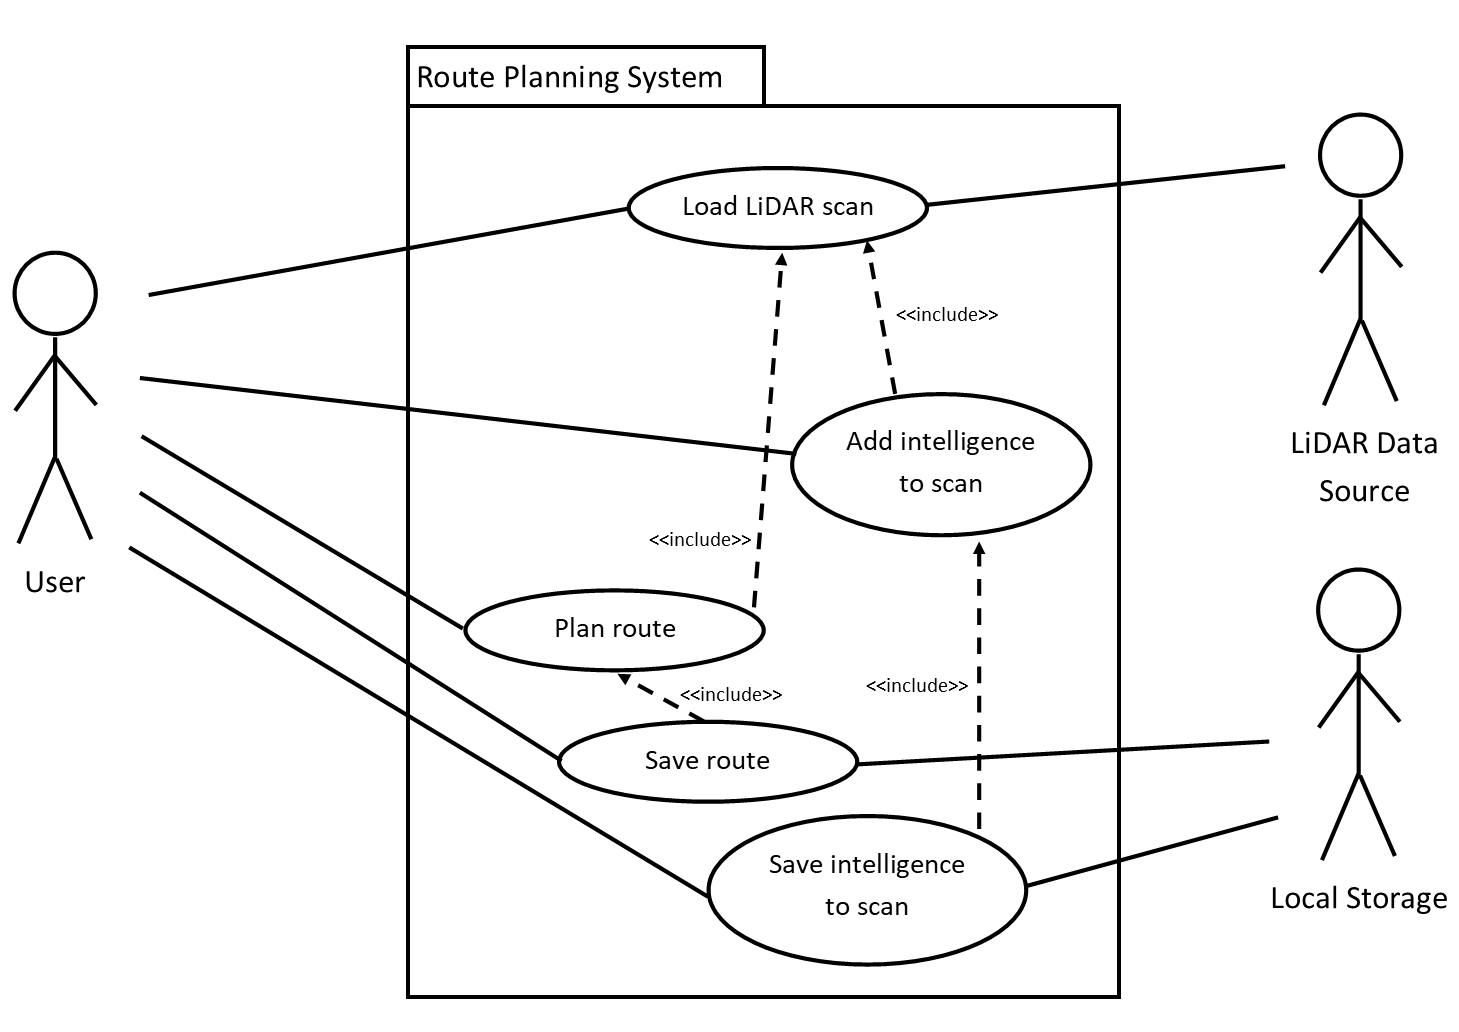
\includegraphics[width=0.85\textwidth]{use_case_diagram}
%     \caption{Use case diagram for project system}
%     \label{use_case_diagram_fig}
%   \end{figure}
%
%   \begin{table}[H]
%     \caption{Functional Requirements}
%     \label{fr_table}
%     \centering
%     \begin{tabular}{|c|c|c|}
%       \hline
%       \textbf{ID} & \textbf{Requirement} & \textbf{Priority} \\ \hline
%       FR1 & Environment agency data can be interpreted & High \\ \hline
%       FR2 & Terrain mesh is generated from LiDAR data & High \\ \hline
%       FR3 & Terrain is rendered to display variations in height & High \\ \hline
%       FR4 & Valid route can be found between specified points & High \\ \hline
%       FR5 & Route can be plotted onto rendering of terrain & High \\ \hline
%       FR6 & Terrain features can be categorised into types & Medium \\ \hline
%       FR7 & Potential for cover is added into rendering & Medium \\ \hline
%       FR8 & Likelihood for enemy attack is accounted for in route & Medium \\ \hline
%       FR9 & Shadows and silhouettes are rendered onto terrain & Low \\ \hline
%       FR10 & Advanced route parameters are taken into account & Low \\ \hline
%     \end{tabular}
%   \end{table}
%
%   \begin{table}[H]
%     \caption{Non-Functional Requirements}
%     \label{nfr_table}
%     \centering
%     \begin{tabular}{|c|c|c|}
%       \hline
%       \textbf{ID} & \textbf{Requirement} & \textbf{Priority} \\ \hline
%       NFR1 & The system can run on a low-powered laptop without stuttering & Medium \\ \hline
%       NFR2 & Users can interact with the system intuitively and with limited literacy & Medium \\ \hline
%       NFR3 & Routes suggested avoid danger as far as possible & High \\ \hline
%       NFR4 & Routes suggested are efficient in terms of exertion & High \\ \hline
%     \end{tabular}
%
%   \end{table}
%
%   \subsection{Equipment Used}
%   \noindent To get the initial LiDAR data, the Environment Agency used an airborne LiDAR scanner, however if the system were to be used in its intended purpose, there are commercially available LiDAR pods to be fixed to standard commercial drones as well as manned aircraft. This provides choice and limits cost to gain an accurate representation of the terrain. The LiDAR files provided have a header detailing the size, resolution and location of the area represented. After the header is a space / newline separated grid of height values to 2 decimal places.
%   \par The primary development machine will be a laptop, due to its availability and its more realistic likeness to the situation that the system is likely to be used in. On the field, the worst-case scenario (which the system must be built around) will be a low-powered laptop without a dedicated graphics card, similar to the development machine. As a result, the project will naturally steer towards graphical efficiency, due to the inconvenience to the development if the rendering has a low framerate.
%   \par To prototype a document parser quickly and check basic functionality, Python was used due to its ease of rapid development. While Python is great for simple proof-of-concept development, it was not designed to perform efficient graphical rendering. The options for a final development language were either C++ or Java; C++ offers unrivalled performance on Windows machines due to its low-level compilation and direct access to OpenGL libraries, while Java can be run on all major platforms with simple setup and is arguably easier to develop on. After considering the options, Java was selected as the language that the system would be built on as versatility and the prospect of fewer blockers in the development cycle appeal more than marginal efficiency gains for this style of project.
%   \par Once a language was finalised, the next choice was which library to use to create the rendering of the terrain. The choice basically boiled down to a low-level graphics library, such as OpenGL or a high-level game engine, such as Unity. A low-level library would allow development of only what is absolutely necessary for the system however would be more complex to implement as all aspects of the engine would need to be built from the ground up. A game engine would streamline the development process, however the end result could end up being bloated with many unnecessary additions, which would require a more powerful machine to run. The LightWeight Java Game Library (LWJGL) was selected as the graphics library that offered the best compromise, as it allows Java to use OpenGL functions, which will keep the computer load to a minimum assuming the correct software engineering practices are followed, while providing opportunity to implement any possible features that the system could require.
%
%   \subsection{System Architecture}
%   \noindent The main requirements for the system are to be able to take in LiDAR data files, render the files for viewing, find an appropriate route through the terrain, and interact with the user. To read the LiDAR data files, a custom parser class will be created for the format of the data supplied by the Environment Agency, however this class will be decoupled as far as possible from the rest of the system so that if the system is deployed after this project then it would be simple for a software engineer to write an equivalent class to parse the file format that they choose to use. On top of the stock LiDAR data, the system will be capable of storing additional intelligence from the user, so the next class in the system will be responsible for pairing the intelligence file with its respective location in the LiDAR scan. This does not need to be as lightly coupled as the LiDAR scan parser as the file format will be defined in this project and should not need to be modified extensively if the LiDAR source changes format.
%   \par Once we have all relevant data within the system, we need to create a terrain mesh to be rendered from the LiDAR points. To do this, a mesh generator class will be written to convert the points into easily-rendered triangles, and pass the mesh to a render engine package to colour the vertices and the fragments using OpenGL functions through the LWJGL. Initially, no extra graphical processing will be done so that computational load is kept to a minimum, allowing the system to be run smoothly on any modern machine. When available, multiple scan resolutions can be used to limit the intensity of rendering by allowing nearby areas to be rendered accurately and far away areas to be less detailed. Later in the information flow, the render engine will be given a route to add to the terrain rendering, which will be represented as a change in colour on the surface of the terrain. While this may cause issues with users that have colour-blindness, the alternative when displaying the route would be to create an elevation change in the model, however doing so would cause a misrepresentation of the land and false information could be taken from viewing the landscape as a result.
%   \par The route-finding element of the system will require a weighted directed graph with weights based on the exertion for a group to move between the locations. The computation required to convert the render mesh into the graph is comparable to starting again from the raw LiDAR points, however the latter it is a shorter, more easily understandable pipeline. Consequently, a graph generator class will be created to take the point cloud and pass the subsequent graph to a route handler class. This route handler will act as an organiser for multiple route finding algorithm classes, conveying start and end points as well as other route preferences, while choosing which algorithm to use. The algorithm classes will purely be concerned with finding the best possible route based on a number of heuristics concerning the enemy evasion aspect of the problem.
%   \par Finally, the system will need a user interaction handler to allow the user\textquotesingle s commands take precedence over all other computation. This handler will be able to convert the commands into actions within the system and send messages across the classes to wherever they need to be acted on. The user interface will require careful consideration due to the limited literacy assumption being made in this project. Any user will need to be able to load a scan, input intelligence such as known enemy locations, known roads, tried and tested safe routes, friendly locations, etc. as well as setting start and end points for the route, and other parameters such as enemy threat and time criticality. Once intelligence has been entered, it should be able to be saved.
%   \par Once a stable build of the system is completed, a single .jar executable can be created, which will allow usage over a broad range of machines on any common Operating System. A diagram showing information flow between entities in the system can be found in Figure \ref{class_diagram_fig}.
%
%
%   \begin{figure}[h]
%     \centering
%     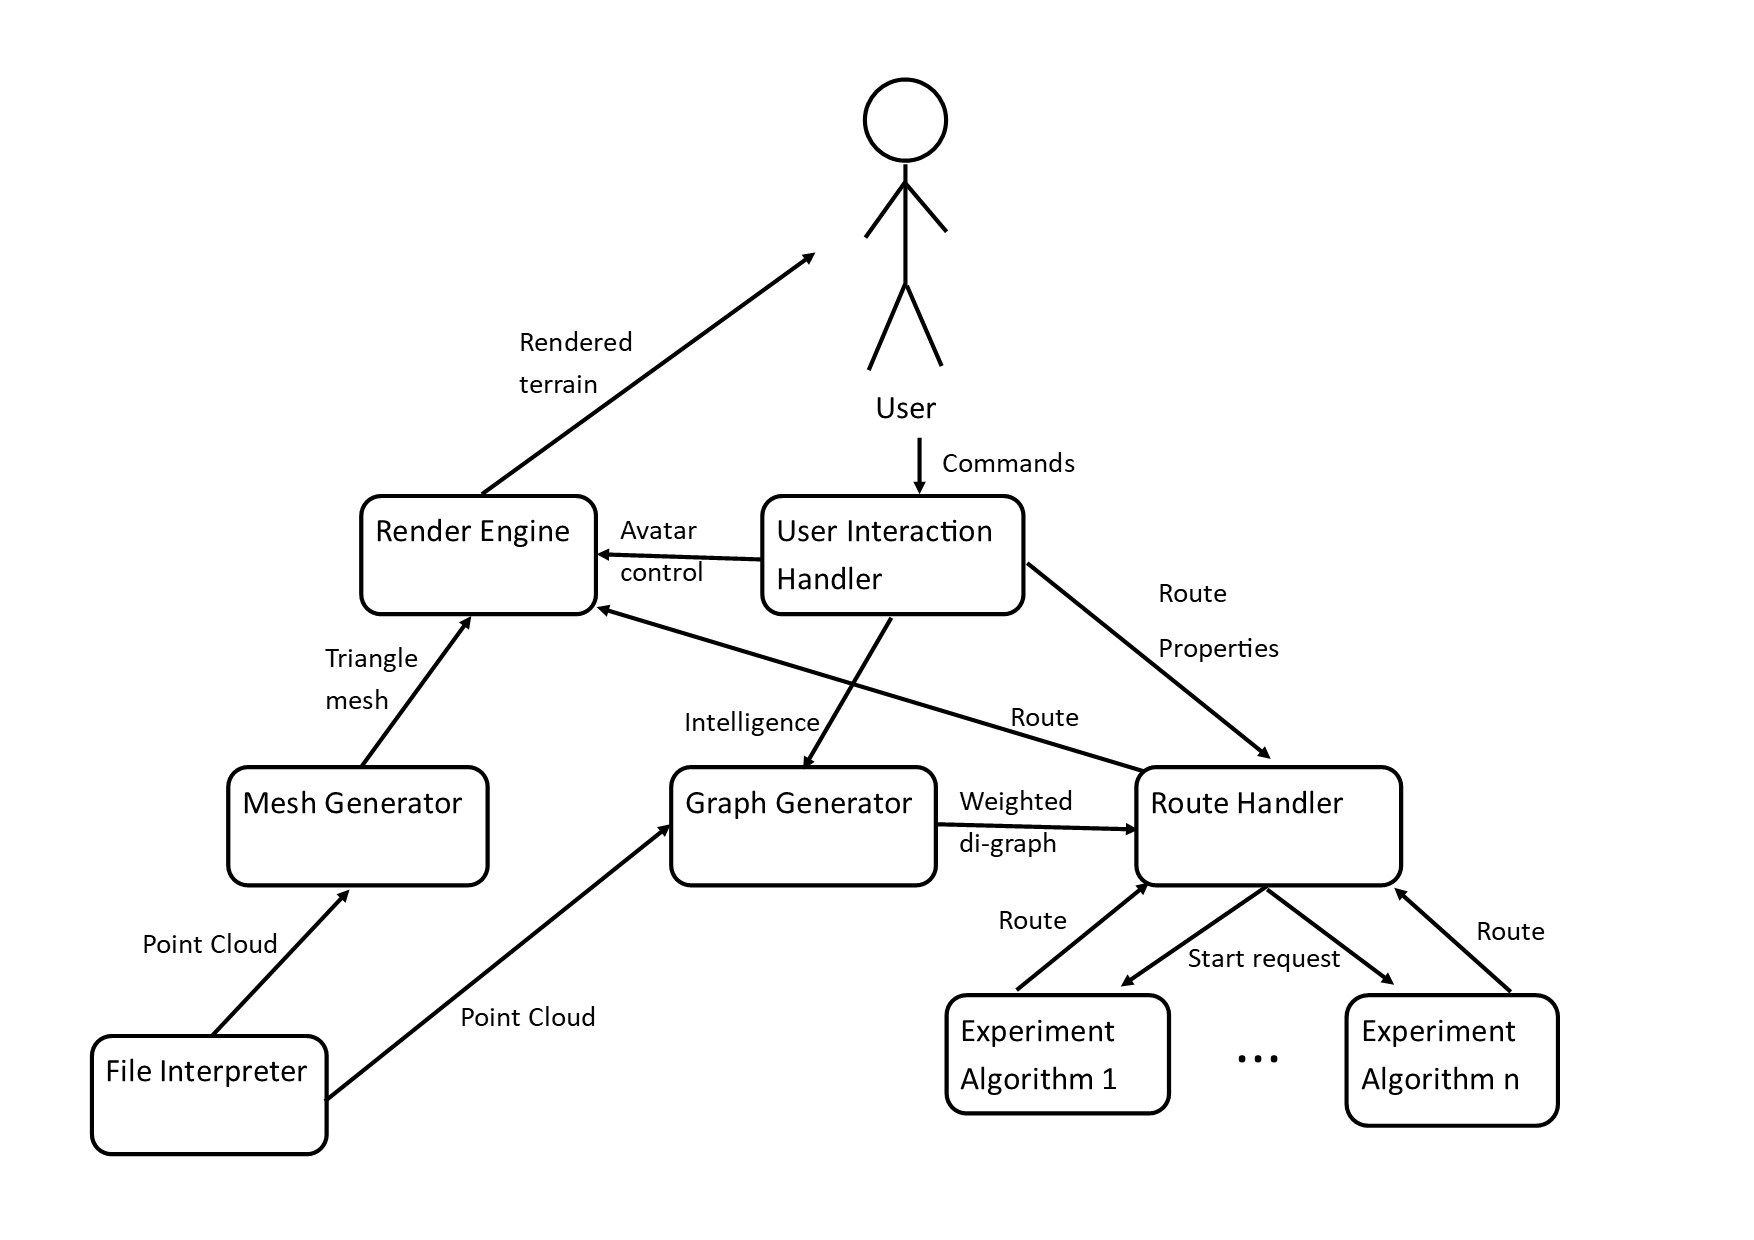
\includegraphics[width=0.9\textwidth]{class_diagram}
%     \caption{Diagram of system components and information flow between them}
%     \label{class_diagram_fig}
%   \end{figure}
%
%   \subsection{User Interaction}
%   \noindent The system will first require the user to load a LiDAR data file. This will be converted into a mesh on loading, which will not be saved to save storage space, as currently a 1 metre resolution scan of 1 km$^2$ is roughly 6MB. Therefore, a full scan of the UK could be estimated at 1.4TB of data, meaning that a complete offline copy of a theatre of operation could feasibly be carried in an external hard drive, however the cost for storing a mesh over a point cloud would tip this possibility over the edge of reasonable.
%   \par Once the mesh has been loaded, the user will be able to access additional intelligence input tools, which will have optional parameters such as intel expiry time for situations such as if an enemy has been temporarily sighted in an area to avoid. When the user is happy with the intelligence on the system, they will be able to save all permanent intelligence into a separate file within the system\textquotesingle s data storage. Alternatively, if there has previously been intelligence on the area loaded to render, then the system will be able to match the files and create a complete picture from the start.
%   \par With the terrain updated to show the latest intelligence, the user will be able to assign start, end, and waypoints to their route as well as optionally tweaking parameters detailing what weight some simplified parameters should be given (threat level, time constraint, etc.). The system will then be set computing an optimal route based on all information at its disposal. Upon completion, the route will be rendered onto the terrain in a colour to make it stand out from the model and the user will be able to walk through the virtual world using the WASD and arrow keys, as in Figure \ref{terrain_fig}.
%
%   \begin{figure}[htb]
%     \centering
%     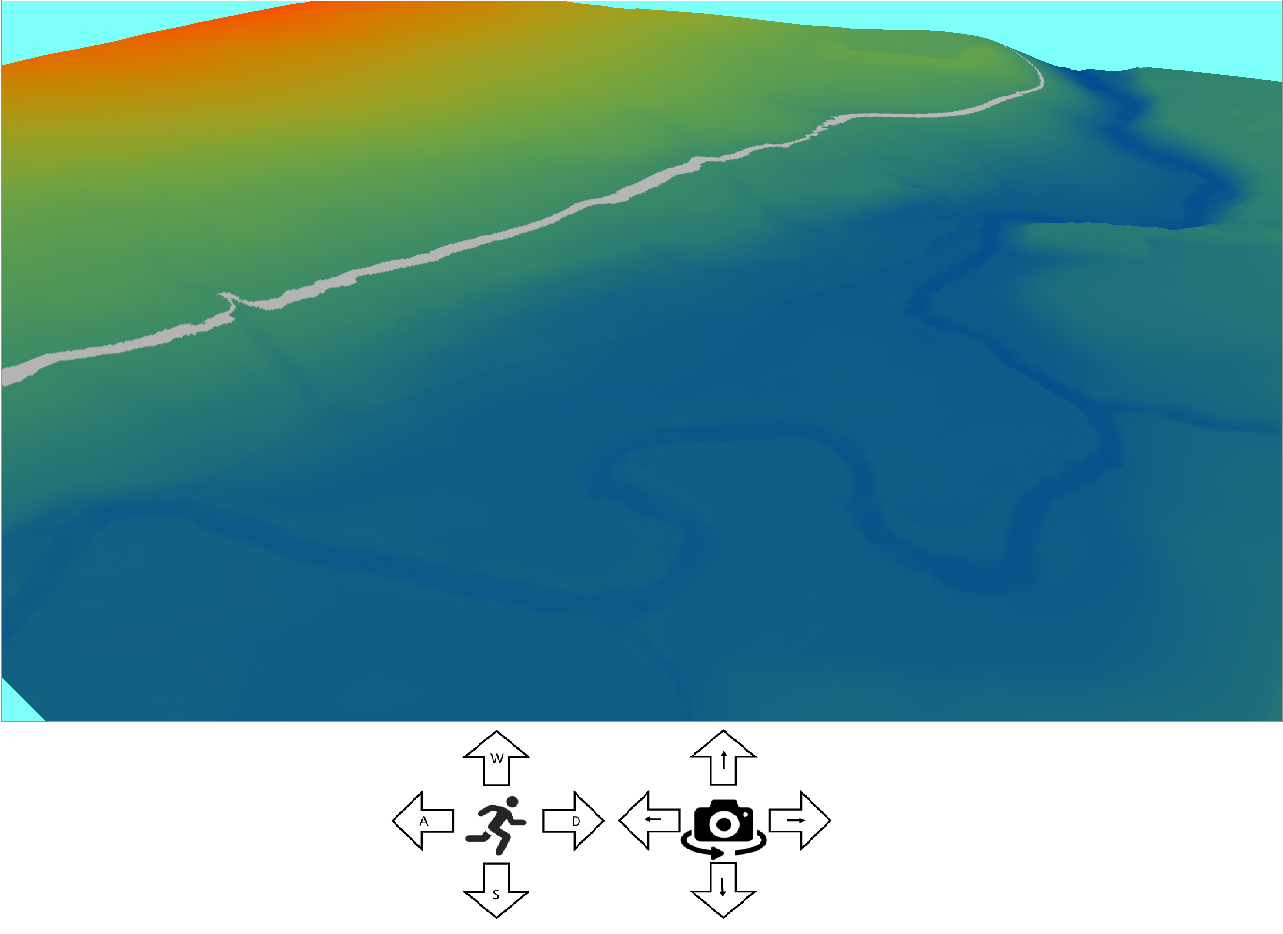
\includegraphics[width=0.75\textwidth]{terrain_reconstruction}
%     \caption{Reconstruction from proposed system indicating path to follow in white with basic user instructions}
%     \label{terrain_fig}
%   \end{figure}








%
%   \subsection{Algorithms}
%   \noindent For a successful project, algorithms will need to be created and optimised to generate a surface mesh from the point cloud data and to find a suitable route through the terrain.
%   \par The Environment Agency LiDAR scan is presented in a regular grid form, so the use of advanced reconstruction algorithms such as the Cocone Algorithm do not provide any useful improvement in output for their extra cost in computation, since it is designed to create a surface from unorganised point clouds, whereas the provided dataset uses organised points in a grid. As a result, a dot to square to triangle approach will be used as is shown in Figure \ref{dot_square_triangle_fig}. Edges are created between neighbouring points to form a regular square grid across the model. Next, for each square in the grid, opposite corners are compared, and the diagonal with the lowest difference in height is selected to turn the square into two easily-rendered triangles while also providing the most natural bending point for the difficult to render 4-point polygon.
%   \begin{figure}[htb]
%     \centering
%     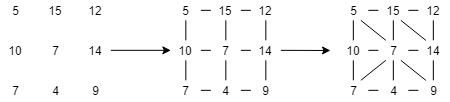
\includegraphics[width=0.75\textwidth]{dot_square_triangle}
%     \caption{Visualisation for dot-square-tringle mesh generation}
%     \label{dot_square_triangle_fig}
%   \end{figure}
%   \par In the dataset, there are many locations (particularly in the DSM) that are null-valued. In an attempt to limit the impact of these null areas, the reconstruction algorithm will find the surface area of the null patch and compare it to a threshold. If the surface area is above the threshold, then to assume anything about that location would be dangerous as an advantageous feature for an enemy to occupy or an impassable object could be there however we would have no way of knowing. The safest thing to do is label this area as a potential risk and attempt to avoid coming close to it. If, on the other hand, the surface area is below the threshold then it should be safe to assume that no significant threat can reside in such a small area and so it would be better to interpolate likely values for the null-valued area to aid route planning.
%   \par The algorithm that will be used to generate a route could be deterministic, such as A* search, or non-deterministic, such as a genetic approach. A* search would be provably optimal as long as we use admissible heuristics, \cite{hart1968formal} however the algorithmic complexity would mean that calculating a route over large distances would take an unreasonable amount of time. Genetic algorithms do not guarantee an optimal, or even a good solution, however probabilistically speaking, with enough generations, they are likely to provide a near-optimal solution while taking a much shorter time to compute than A* search. Additionally, if an A* based algorithm is the only one developed, then a change to the specification of the algorithm could be very difficult to implement. Genetic algorithms are extremely good at handling all kinds of problems, so adding extra features should not require much work.
%   \par Traditionally, these algorithms are used to find shortest path solutions to directed or undirected graphs. The use case for this system requires that the algorithms are modified to use a number of different analytical parameters, each with a weight that can be changed by the user to suit the situation of the mission.
%   \par Without being able to test the performance of each algorithm, there is no way to choose a single route that will certainly be the best. Both algorithms will be developed in parallel and once both are working as well as possible, they can be compared in terms of route optimality, memory used and computation time to decide ultimately which will be most effective in the final system, or if both have situations that they excel at and it would be worthwhile to keep both algorithms in the final product.
%
% \section{Testing and Evaluation}
% \noindent The quality of the system will be quantified by metrics that need to measure the accuracy of reconstruction, the effectiveness of the route planned, and the burden on the system that runs it.
% \par Reconstruction accuracy can be checked by visualising a possible route through an easily identifiable area, such as the Lake District, and recording a video of a real-world hike through the terrain. By showing both representations side-by-side, we can compare the likeness produced by the system to the real thing.
% \par Route effectiveness would be best quantified by a score awarded by an expert in the field. As the effectiveness is such a subjective topic, the expert will be asked to experiment with the user-defined parameters before giving an opinion so that the system has chance to adapt to their personal preference. Coupling expert opinion with comparisons with existing hiking route finding applications should give a clear indication of the success of the project in creating a good route.
% \par To test system burden, the final product will be run on a laptop without a dedicated graphics card, and the CPU and memory usage will be recorded as well as the system temperature. If the laptop can run the system continuously for a specified period of time, while maintaining reasonable resource usage and temperature, then the system will pass the test. Comparisons to existing applications may not be possible as trends in computationally expensive tasks are tending towards offering a solution as Software as a Service (SaaS), meaning that the best systems will not burden the local machine with the task of computing the route. From the use case of this project, it will not be possible to host this software in SaaS as reliable internet connections can not be relied on in combat situations.

\bibliography{bibliography}


\end{document}
